\section{Results}
\label{sec:results}
All 840 selected probes (2 datasets $\times$ 2 encoders $\times$ 3 splits $\times$ 10 draws $\times$ 7 arms) passed the completeness and provenance audit, and every selected fit converged. No bootstrap replicate lacked test support for a class. The Virchow2 arms reproduce the earlier estimates on fresh training draws: $D_R$ at $\rho=100$ is 3.15 points on TCGA-UT against 2.91 before, and 7.86 points on BRACS against 7.65 \citep{queisler2026prevalenceTcga, queisler2026prevalenceBracs}. The decomposition identity $\delta_R=\delta_P+\delta_S+\delta_I$ holds exactly by construction.

\subsection{Balanced and imbalanced accuracy}
Absolute accuracy comes first, so that a damage contrast is not read through a floor effect. On TCGA-UT, UNI2-h is more accurate than Virchow2 under balanced training, by 1.78 points (95\% interval $[1.26, 2.30]$), and the advantage grows to 2.64 points $[2.12, 3.17]$ at $\rho=100$ (Figure~\ref{fig:accuracy}, left). On BRACS, UNI2-h is 1.32 points less accurate under balanced training, with an interval of $[-3.08, 0.63]$ that includes zero, and 0.65 points $[-1.75, 0.36]$ less accurate at $\rho=100$. Neither BRACS difference is resolved. Both encoders stay near 38 to 40 percent balanced accuracy on seven BRACS classes and near 72 to 74 percent on thirty TCGA-UT classes, so the dataset, not the encoder, sets the accuracy level.

\begin{figure}[t]
  \centering
  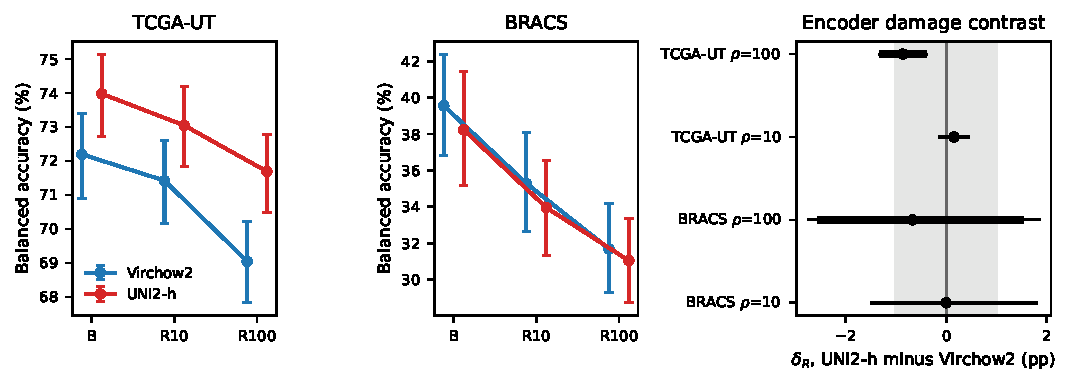
\includegraphics[width=\textwidth]{fig_accuracy_damage.pdf}
  \caption{UNI2-h reduces the $\rho=100$ damage on TCGA-UT while starting from a higher balanced accuracy; on BRACS neither the accuracy levels nor the damage contrast are resolved. Left and centre: test patient-macro balanced accuracy of the balanced arm B and the ratio arms R10 and R100, with paired 95\% intervals. Right: encoder contrast $\delta_R$ of the damage $D_R$; negative values mean less damage with UNI2-h. Thick bars are 95\% intervals, the thin bar on each $\rho=100$ row is the primary two-sided 97.5\% interval, and the grey band marks the $\pm 1$-point practical threshold.}
  \label{fig:accuracy}
\end{figure}

\subsection{Primary damage contrast}
On TCGA-UT, UNI2-h loses 2.29 points at $\rho=100$ and Virchow2 3.15 points. The primary contrast is $\delta_R=-0.86$ points with a 97.5\% interval of $[-1.33, -0.40]$. The interval excludes zero, so the direction is resolved: UNI2-h loses less balanced accuracy under this imbalance. It neither lies wholly below $-1$ point nor wholly inside $[-1,+1]$, so the decision rule leaves open whether the reduction is practically meaningful. All three splits agree in sign and size, with observed contrasts between $-0.93$ and $-0.81$ points (Table~\ref{tab:splits}). Because UNI2-h is also the more accurate encoder at both B and R100, the smaller damage is not an artefact of a lower baseline.

On BRACS, UNI2-h loses 7.19 points and Virchow2 7.86 points. The contrast is $\delta_R=-0.67$ points with a 97.5\% interval of $[-2.75, 1.85]$, which includes zero and both practical thresholds: the BRACS outcome is unresolved. The splits disagree, from $+0.79$ to $-3.13$ points, and the draw standard deviation of $D_R$ within a split is 2.3 to 3.9 points on either encoder, so this design cannot distinguish a moderate BRACS reduction from none. At the moderate ratio $\rho=10$, the damage is almost identical for both encoders: $\delta_R=0.16$ $[-0.11, 0.44]$ on TCGA-UT and $-0.00$ $[-1.47, 1.79]$ on BRACS (Table~\ref{tab:decomp10}).

\subsection{Which operational channel changed}
Table~\ref{tab:decomp} splits the $\rho=100$ damage into its prior, support, and interaction parts. On TCGA-UT the prior-only damage is not reduced: $\delta_P=0.24$ $[-0.06, 0.54]$. The reduction comes from the support-only damage, $\delta_S=-0.37$ $[-0.55, -0.18]$, and above all from the interaction, $\delta_I=-0.74$ $[-0.99, -0.50]$: on Virchow2 the prior and support channels compound by 1.17 points beyond their sum, on UNI2-h by only 0.43 points. On BRACS, UNI2-h again carries less support-only damage, $\delta_S=-1.67$ $[-2.92, -0.52]$, but a larger interaction, $\delta_I=1.62$ $[0.15, 3.21]$, cancels most of that reduction, and the prior contrast $\delta_P=-0.62$ $[-2.31, 1.37]$ is unresolved.

\begin{table}[t]
  \centering
  \footnotesize
  \setlength{\tabcolsep}{4pt}
  \begin{tabular}{lcccccc}
    \toprule
    & \multicolumn{3}{c}{Tuned $\lambda$ per arm (primary)} & \multicolumn{3}{c}{B-selected $\lambda$ (sensitivity)} \\
    \cmidrule(lr){2-4}\cmidrule(lr){5-7}
    & Virchow2 & UNI2-h & UNI2-h $-$ Virchow2 & Virchow2 & UNI2-h & Diff. \\
    \midrule
    \tabinput{tab_decomposition_100.tex}
    \bottomrule
  \end{tabular}
  \caption{On both datasets UNI2-h carries less support-only damage under either regularization rule, whereas the total and the interaction contrasts depend on how $\lambda$ is chosen. Damage components at $\rho=100$ in balanced-accuracy points, defined in Equation~\eqref{eq:damage}, with paired 95\% intervals; the primary contrast's 97.5\% interval is given in the text. The right block re-evaluates each encoder's stored P100, S100, and R100 candidates at that encoder's own B-selected $\lambda$, per split and draw; it has no intervals.}
  \label{tab:decomp}
\end{table}

The decomposition must also survive the choice of regularization. When every arm is held at its encoder's B-selected $\lambda$, both encoders lose far more accuracy, mainly through the prior arm, and the ordering of total damage reverses: UNI2-h then loses 6.73 points more than Virchow2 on TCGA-UT and 3.27 points more on BRACS (Table~\ref{tab:decomp}, right). The TCGA-UT interaction reduction also disappears under that rule. Only the support-channel contrast keeps its sign under both rules on both datasets, at $-0.44$ and $-1.51$ points under the fixed rule. The tuned primary result is therefore a statement about the full pipeline, in which each encoder's probe re-selects its penalty for each imbalanced training set; it is not a statement that UNI2-h's features resist a shifted prior at a common regularization strength. The penalty scale is not comparable across encoders either: UNI2-h's validation features have mean Euclidean norms of 16.9 (TCGA-UT) and 15.3 (BRACS), against 49.4 and 46.4 for Virchow2 (Table~\ref{tab:validation}), so one numerical $\lambda$ regularizes the two encoders to a different degree.

\subsection{Probability quality}
Table~\ref{tab:prob} reports macro NLL and ECE at B and R100. Raw UNI2-h probabilities are less well calibrated under balanced training on both datasets: ECE is about 10 points higher, and the fitted temperatures of 0.65 (TCGA-UT) and 0.56 (BRACS), below one, show that the raw probabilities are underconfident. Temperature scaling removes most of that gap. After scaling, UNI2-h has the lower NLL on TCGA-UT at both B ($-0.06$ nats $[-0.08, -0.04]$) and R100, while on BRACS its balanced NLL remains 0.06 nats $[0.02, 0.10]$ higher. The imbalance damage in scaled NLL is slightly smaller for UNI2-h on both datasets, by 0.03 nats $[-0.04, -0.02]$ on TCGA-UT and 0.08 nats $[-0.11, -0.04]$ on BRACS. The large reduction in raw ECE damage on TCGA-UT, $-7.72$ points $[-11.01, -4.35]$, mostly reflects UNI2-h's poorly calibrated balanced starting point, not better calibration under imbalance: after scaling, the damage contrast in ECE is $0.57$ points $[-0.06, 1.15]$.

\begin{table}[t]
  \centering
  \footnotesize
  \setlength{\tabcolsep}{4pt}
  \begin{tabular}{lcccccc}
    \toprule
    & \multicolumn{2}{c}{B} & \multicolumn{2}{c}{R100} & \multicolumn{2}{c}{UNI2-h $-$ Virchow2} \\
    \cmidrule(lr){2-3}\cmidrule(lr){4-5}\cmidrule(lr){6-7}
    & Virchow2 & UNI2-h & Virchow2 & UNI2-h & at B & in damage R100$-$B \\
    \midrule
    \tabinput{tab_probability_R100.tex}
    \bottomrule
  \end{tabular}
  \caption{Raw UNI2-h probabilities start less well calibrated, and after temperature scaling the imbalance damage in probability quality is similar for both encoders. Macro NLL in nats and ECE in percentage points, raw and after validation temperature scaling, with paired 95\% intervals for the encoder contrasts. The damage contrast compares each encoder's R100-minus-B change. Ratio 10 is in Table~\ref{tab:prob10}.}
  \label{tab:prob}
\end{table}

\subsection{Where the damage lands}
On TCGA-UT the lower damage shows in the tail. The tail third of classes, by assigned rank, loses 12.5 points of recall on Virchow2 at $\rho=100$ but 7.1 points on UNI2-h, while the head third gains 5.3 and 2.3 points (Table~\ref{tab:thirds}). On BRACS both encoders collapse the tail third to about 9 to 10 percent recall, from about 41 percent under balanced training, so the tail offers no room for an encoder difference. Per class, averaged over the ranks each class visits across draws, 22 of the 30 TCGA-UT classes lose less recall with UNI2-h; on BRACS 4 of 7 do, with differences of several points in both directions (Figure~\ref{fig:perclass}). The validation diagnostics are consistent with this split between datasets but do not explain it. On TCGA-UT, UNI2-h has the higher validation balanced accuracy (74.2 against 72.3 percent) and a larger standardized validation margin (0.72 against 0.64), where the margin is the true-class logit minus the strongest competing logit, divided by that model's validation margin standard deviation. On BRACS, UNI2-h has the lower validation accuracy (42.2 against 43.4 percent) and a margin near zero (0.05 against 0.15). The most confused class pairs are the same for both encoders: colon against rectal adenocarcinoma on TCGA-UT, and ADH and DCIS predicted as FEA and PB against N on BRACS. These comparisons remain exploratory, because the encoders differ in architecture, dimension, training data, and pooling at the same time.

\section{Discussion}
\label{sec:discussion}
\textbf{Did balanced performance change?} On TCGA-UT, yes: UNI2-h is 1.78 points more accurate under balanced training. On BRACS the difference, $-1.32$ points, is unresolved.

\textbf{Did imbalance damage change?} On TCGA-UT the direction is resolved: under the tuned pipeline UNI2-h loses 0.86 points less balanced accuracy at $\rho=100$, consistently across the three splits, while also being more accurate at both ends. Whether that reduction is practically meaningful is unresolved, because the primary interval straddles the one-point threshold. On BRACS the primary contrast is unresolved. It does not support practical similarity either, because its interval extends beyond both thresholds. At $\rho=10$ the two encoders lose almost the same accuracy on both datasets, so any encoder difference emerges only at severe imbalance. The large-damage regime of BRACS, a 7-to-8-point loss with a collapsed tail, is therefore not a Virchow2 peculiarity: a second encoder with different pretraining data and pooling shows the same regime.

\textbf{Which operational channel changed?} The only contrast that holds its sign on both datasets and under both regularization rules is a smaller support-only damage for UNI2-h: with a uniform class prior, redistributing patches toward the head costs UNI2-h less accuracy. The prior-only damage is not reduced under tuned regularization, and the interaction behaves differently on the two datasets: smaller on TCGA-UT, larger on BRACS, where it absorbs the support reduction. Under a fixed, B-selected penalty the prior damage of UNI2-h becomes much larger, which shows that the tuned result depends on each imbalanced probe re-selecting a weaker penalty. These are statements about the operational prior and support channels of the fitted pipeline. They do not identify a biological or representational mechanism; establishing feature geometry as a causal mediator would need a separate intervention that changes geometry while holding the encoder fixed.

\textbf{Limitations.} The study compares two encoders with one linear readout on fixed patients and fixed splits; the results do not generalize to foundation models as a category. The two datasets use different support budgets, so the BRACS--TCGA-UT difference is descriptive. The encoders differ in native embedding width, transform, pooling, and pretraining data at once, and the report cannot attribute a contrast to any one of them. The public descriptions of both encoders' pretraining data were not audited against the TCGA-UT and BRACS source slides beyond reading the UNI2-h model card, so undocumented overlap cannot be excluded. The intervals condition on the available test patients, which earlier studies in this series have already examined. The B-selected-$\lambda$ sensitivity has point estimates only.
